
   \chapter{File system}   
    \label{CH:FS}     

文件系统的目的是组织和存储数据。文件系统通常支持用户和应用程序之间的数据共享,以及
    \indextext{persistence}   ,以便数据在重新启动后仍然可用。  

xv6 文件系统提供类 Unix 的文件、目录和路径名(请参阅第    \ref{CH:UNIX}    章),并将其数据存储在 virtio 磁盘上以实现持久性。文件系统解决了几个挑战:
    \begin{itemize}

 
   \item   文件系统需要磁盘上的数据结构来表示命名目录和文件的树,记录保存每个文件内容的块的标识,并记录磁盘的哪些区域是空闲的。   \item   文件系统必须支持
    \indextext{crash recovery}    。也就是说,如果发生崩溃(例如电源故障),文件系统在重新启动后仍必须正常工作。风险在于崩溃可能会中断一系列更新并留下不一致的磁盘数据结构(例如,既在文件中使用又标记为空闲的块)。   \item   不同的进程可能同时对文件系统进行操作,因此文件系统代码必须协调以保持不变量。   \item   访问磁盘比访问内存慢几个数量级,因此文件系统必须维护常用块的内存缓存。  \end{itemize}     

本章的其余部分将解释 xv6 如何应对这些挑战。
    \section{概述  }     

xv6 文件系统实现分为七层,如图    \ref{fig:fslayer}    所示。磁盘层在 virtio 硬盘驱动器上读取和写入块。缓冲区缓存层缓存磁盘块并同步对它们的访问,确保一次只有一个内核进程可以修改存储在任何特定块中的数据。日志记录层允许高层将多个块的更新包装在一个
    \indextext{transaction}    ,并确保在崩溃时自动更新块(即全部更新或不更新)。 inode 层提供单独的文件,每个文件表示为
    \indextext{inode}    具有唯一的 i-number 和一些保存文件数据的块。目录层将每个目录实现为一种特殊的索引节点,其内容是一系列目录条目,每个目录条目包含一个文件名和 i-number。路径名层提供分层路径名,例如
    \lstinline{/usr/rtm/xv6/fs.c}    ,并通过递归查找来解析它们。文件描述符层使用文件系统接口抽象许多 Unix 资源(例如管道、设备、文件等),简化了应用程序程序员的工作。  

   \begin{figure}[t]
\center
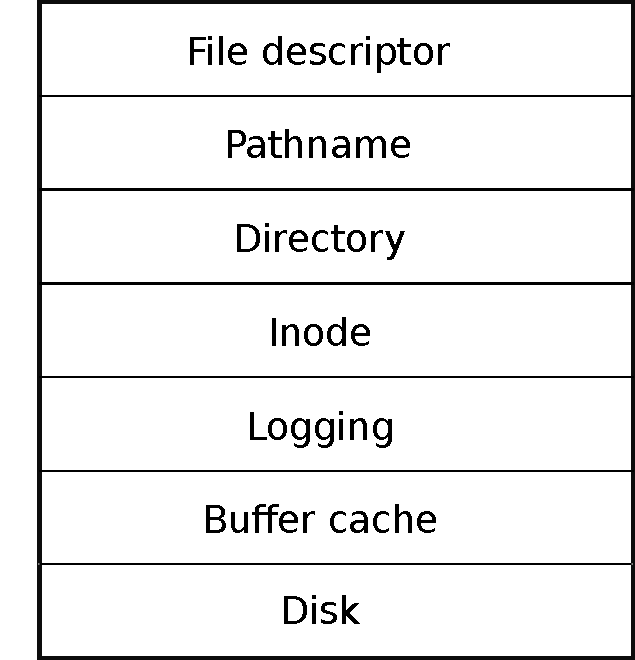
\includegraphics[scale=0.5]{fig/fslayer.pdf}
\caption{xv6 文件系统的层。  }
\label{fig:fslayer}
\end{figure}     

磁盘硬件传统上将磁盘上的数据呈现为 512 字节块的编号序列
    \index{block}   (也称为扇区):
    \index{sector}    扇区 0 是前 512 个字节,扇区 1 是下一个字节,依此类推。操作系统用于其文件系统的块大小可能与磁盘使用的扇区大小不同,但通常块大小是扇区大小的倍数。 Xv6 保存已读入内存的块的副本(类型为对象)
    \lstinline{struct buf}   
    \lineref{kernel/buf.h:/^struct.buf/}    。此结构中存储的数据有时与磁盘不同步:它可能尚未从磁盘读入(磁盘正在处理它,但尚未返回扇区的内容),或者它可能已被软件更新但尚未写入磁盘。  

文件系统必须计划在磁盘上存储 inode 和内容块的位置。为此,xv6 将磁盘分为几个部分,如图~\ref{fig:fslayout}    所示。文件系统不使用块 0(它保存引导扇区)。块 1 称为
    \indextext{superblock}   ;它包含有关文件系统的元数据(文件系统大小(以块为单位)、数据块数量、索引节点数量以及日志中的块数量)。从 2 开始的块保存日志。日志之后是索引节点,每个块有多个索引节点。之后是位图块,跟踪哪些数据块正在使用。其余块为数据块;每个都在位图块中标记为空闲,或者保存文件或目录的内容。超级块由一个单独的程序填充,称为
    \indexcode{mkfs}    ,构建初始文件系统。  

本章的其余部分将讨论每一层,从缓冲区高速缓存开始。留意较低层精心选择的抽象有助于较高层设计的情况。
    \section{缓冲区高速缓存层  }   
    \label{s:bcache}     

缓冲区高速缓存有两个工作:(1)同步对磁盘块的访问,以确保内存中只有一个块的副本,并且一次只有一个内核线程使用该副本; (2) 缓存流行的块,这样就不需要从慢速磁盘重新读取它们。代码在
    \lstinline{bio.c}    。  

buffer cache导出的主要接口包括
    \indexcode{bread}    和
    \indexcode{bwrite}    ;前者获得
    \indextext{buf}    包含可以在内存中读取或修改的块的副本,后者将修改后的缓冲区写入磁盘上的相应块。内核线程必须通过调用释放缓冲区
    \indexcode{brelse}    完成后。缓冲区高速缓存使用每缓冲区睡眠锁来确保一次只有一个线程使用每个缓冲区(以及每个磁盘块);
    \lstinline{bread}    返回一个锁定的缓冲区,并且
    \lstinline{brelse}    释放锁。  

让我们回到缓冲区高速缓存。缓冲区高速缓存具有固定数量的缓冲区来保存磁盘块,这意味着如果文件系统请求高速缓存中尚未存在的块,则缓冲区高速缓存必须回收当前保存其他块的缓冲区。缓冲区高速缓存为新块回收最近最少使用的缓冲区。假设最近最少使用的缓冲区是最不可能很快再次使用的缓冲区。  

   \begin{figure}[t]
\center
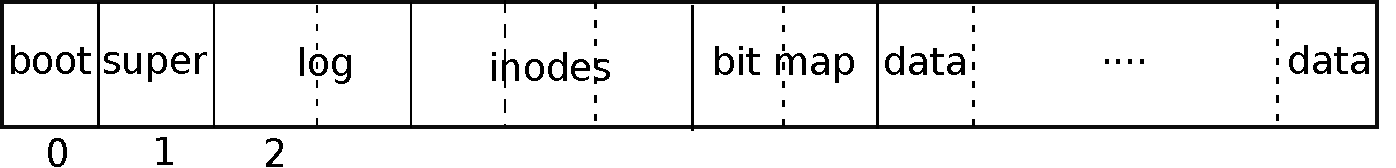
\includegraphics[scale=0.5]{fig/fslayout.pdf}
\caption{xv6 文件系统的结构。  }
\label{fig:fslayout}
\end{figure}   
    \section{代码:缓冲区缓存  }     

缓冲区高速缓存是缓冲区的双向链表。
    \indexcode{main}   
    \lineref{kernel/main.c:/binit/}调用函数\indexcode{binit}    ,使用静态数组     \lstinline{buf} \linerefs{kernel/bio.c:/Create.linked.list/,/^..}/} 中的 NBUF 缓冲区初始化列表。对缓冲区高速缓存的所有其他访问都通过 bcache.head 引用链表,而不是 buf 数组。  

缓冲区有两个与其关联的状态字段。字段
    \indexcode{valid}    指示缓冲区包含该块的副本。字段    \indexcode{disk}    指示缓冲区内容已传递到磁盘,这可能会更改缓冲区(例如,将数据从磁盘写入    \lstinline{data}    )。  

   \lstinline{bread}   
    \lineref{kernel/bio.c:/^bread/}    调用
    \indexcode{bget}    获取给定扇区的缓冲区
    \lineref{kernel/bio.c:/b.=.bget/}    。如果需要从磁盘读取缓冲区,
    \lstinline{bread}    调用
    \indexcode{virtio_disk_rw}    在返回缓冲区之前执行此操作。  

   \lstinline{bget}   
    \lineref{kernel/bio.c:/^bget/}    扫描缓冲区列表以查找具有给定设备号和扇区号的缓冲区
\linerefs{kernel/bio.c:/Is.the.block.already/,/^..}    /}。如果有这样的缓冲区的话
    \indexcode{bget}    获取缓冲区的睡眠锁。
 然后    \lstinline{bget}    返回锁定的缓冲区。  

如果给定扇区没有缓存缓冲区,
    \indexcode{bget}    必须创建一个,可能会重用保存不同扇区的缓冲区。它第二次扫描缓冲区列表,查找未使用的缓冲区 (    \lstinline{b->refcnt = 0}    );可以使用任何此类缓冲区。
    \lstinline{bget}    编辑缓冲区元数据以记录新的设备和扇区号并获取其睡眠锁。请注意,分配
    \lstinline{b->valid = 0}    确保
    \lstinline{bread}    将从磁盘读取块数据,而不是错误地使用缓冲区以前的内容。  

重要的是,每个磁盘扇区最多有一个缓存缓冲区,以确保读取器看到写入,并且因为文件系统使用缓冲区上的锁来进行同步。
    \lstinline{bget}    通过保持
    \lstinline{bache.lock}    从第一个循环检查该块是否已缓存到第二个循环声明该块现在已被缓存(通过设置
    \lstinline{dev}    ,
    \lstinline{blockno}    和
    \lstinline{refcnt}   )。这会导致对块是否存在的检查以及(如果不存在)对保存该块的缓冲区的指定是原子的。  

这是安全的
    \lstinline{bget}    获取缓冲区外部的睡眠锁
    \lstinline{bcache.lock}    临界区,由于非零
    \lstinline{b->refcnt}    防止缓冲区被重新用于不同的磁盘块。睡眠锁保护块缓冲内容的读写,而
    \lstinline{bcache.lock}    保护有关缓存哪些块的信息。  

如果所有缓冲区都忙,则说明有太多进程同时执行文件系统调用;
    \lstinline{bget}    出现Panic。更优雅的响应可能是休眠直到缓冲区空闲,尽管这样可能会出现死锁。  

一次
    \indexcode{bread}    已读取磁盘(如果需要)并将缓冲区返回给其调用者,调用者独占使用该缓冲区并可以读取或写入数据字节。如果调用者确实修改了缓冲区,则必须调用
    \indexcode{bwrite}    在释放缓冲区之前将更改的数据写入磁盘。
    \lstinline{bwrite}   
    \lineref{kernel/bio.c:/^bwrite/}    调用
    \indexcode{virtio_disk_rw}    与磁盘硬件对话。  

当调用者使用完缓冲区后,它必须调用
    \indexcode{brelse}    来释放它。 (名字
    \lstinline{brelse}    是 b-release 的缩写,虽然神秘但值得学习:它起源于 Unix,也用于 BSD、Linux 和 Solaris。)
    \lstinline{brelse}   
    \lineref{kernel/bio.c:/^brelse/}    释放睡眠锁并将缓冲区移动到链表的前面
    \linerefs{kernel/bio.c:/b->next->prev.=.b->prev/,/bcache.head.next.=.b/}    。移动缓冲区会导致列表按照缓冲区最近使用的时间(意味着释放)进行排序:列表中的第一个缓冲区是最近使用的,最后一个缓冲区是最近最少使用的。中的两个循环
    \lstinline{bget}    利用了这一点:在最坏的情况下,对现有缓冲区的扫描必须处理整个列表,但首先检查最近使用的缓冲区(从
    \lstinline{bcache.head}    及以下
 当存在良好的引用局部性时,   \lstinline{next}    指针)将减少扫描时间。选择要重用的缓冲区的扫描通过向后扫描来选择最近最少使用的缓冲区(以下
    \lstinline{prev}    指针)。
    \section{日志层  }     

文件系统设计中最有趣的问题之一是崩溃恢复。出现此问题的原因是许多文件系统操作涉及对磁盘的多次写入,并且写入子集后发生崩溃可能会使磁盘上的文件系统处于不一致的状态。例如,假设在文件截断期间发生崩溃(将文件的长度设置为零并释放其内容块)。根据磁盘写入的顺序,崩溃可能会留下一个带有对标记为空闲的内容块的引用的索引节点,也可能会留下一个已分配但未引用的内容块。  

后者相对良性,但引用已释放块的索引节点在重新启动后可能会导致严重问题。重新启动后,内核可能会将该块分配给另一个文件,现在我们有两个不同的文件无意中指向同一个块。如果 xv6 支持多个用户,这种情况可能会成为安全问题,因为旧文件的所有者将能够读取和写入由不同用户拥有的新文件中的块。  

Xv6 通过简单的日志记录形式解决了文件系统操作期间的崩溃问题。 xv6 系统调用不直接写入磁盘文件系统数据结构。相反,它将它希望进行的所有磁盘写入的描述放在一个
 磁盘上的    \indextext{log}   。一旦系统调用记录了所有写入,它就会写入一个特殊的
    \indextext{commit}    记录到磁盘,表明日志包含完整的操作。此时,系统调用会将写入内容复制到磁盘文件系统数据结构。这些写入完成后,系统调用会擦除磁盘上的日志。  

如果系统崩溃并重新启动,文件系统代码会在运行任何进程之前按如下方式从崩溃中恢复。如果日志被标记为包含完整操作,则恢复代码会将写入内容复制到磁盘文件系统中它们所属的位置。如果日志未标记为包含完整操作,则恢复代码将忽略该日志。恢复代码通过擦除日志来完成。  

为什么xv6的日志解决了文件系统操作崩溃的问题?如果崩溃发生在操作提交之前,则磁盘上的日志将不会被标记为完成,恢复代码将忽略它,并且磁盘的状态将就像操作尚未开始一样。如果崩溃发生在操作提交之后,那么恢复将重放该操作的所有写入,如果该操作已开始将它们写入磁盘数据结构,则可能会重复它们。在任何一种情况下,日志都会使操作相对于崩溃而言是原子的:恢复后,操作的所有写入要么都出现在磁盘上,要么都不出现。
    \section{日志设计  }     

日志驻留在超级块中指定的已知固定位置。它由一个标头块组成,后跟一系列更新的块副本(“记录块”)。标头块包含一组扇区号,每个扇区号对应每个已记录的块,以及日志块的计数。磁盘上标头块中的计数要么为零,表示日志中没有事务,要么非零,表示日志包含具有指定数量的已记录块的完整已提交事务。 Xv6 在事务提交时(而不是之前)写入标头块,并在将记录的块复制到文件系统后将计数设置为零。因此,事务中途崩溃将导致日志标头块中的计数为零;提交后的崩溃将导致非零计数。  

每个系统调用的代码指示写入序列的开始和结束,这些写入序列对于崩溃而言必须是原子的。为了允许不同进程并发执行文件系统操作,日志系统可以将多个系统调用的写入累积到一个事务中。因此,单个提交可能涉及多个完整系统调用的写入。为了避免跨事务分割系统调用,日志系统仅在没有文件系统系统调用正在进行时提交。  

一起提交多个事务的想法被称为
    \indextext{group commit}    。组提交减少了磁盘操作的数量,因为它将一次提交的固定成本分摊到多个操作上。组提交还可以同时为磁盘系统提供更多并发写入,也许允许磁盘在单个磁盘旋转期间将它们全部写入。 xv6的virtio驱动不支持这种
    \indextext{batching}    ,但 xv6 的文件系统设计允许这样做。  

Xv6 在磁盘上指定固定数量的空间来保存日志。事务中系统调用写入的块总数必须适合该空间。这有两个后果。不允许单个系统调用写入多于日志空间的不同块。对于大多数系统调用来说这不是问题,但是其中两个系统调用可能会写入许多块:
    \indexcode{write}    和
    \indexcode{unlink}    。大文件写入可能会写入很多数据块和很多位图块以及一个inode块;取消链接大文件可能会写入许多位图块和一个索引节点。 Xv6 的写入系统调用将大型写入分解为多个适合日志的较小写入,并且
    \lstinline{unlink}    不会引起问题,因为实际上 xv6 文件系统仅使用一个位图块。有限日志空间的另一个后果是日志系统不允许系统调用启动,除非确定系统调用的写入适合日志中的剩余空间。
    \section{代码:记录  }     

系统调用中日志的典型用法如下:
\begin{lstlisting}[]
begin_op();
...
bp = bread(...);
bp->data[...] = ...;
log_write(bp);
...
end_op();
\end{lstlisting}     

   \indexcode{begin_op}   
    \lineref{kernel/log.c:/^begin.op/}    一直等待,直到日志系统当前未提交,并且有足够的未保留日志空间来保存此调用的写入。
    \lstinline{log.outstanding}    统计保留日志空间的系统调用数量;总保留空间为
    \lstinline{log.outstanding}    次
    \lstinline{MAXOPBLOCKS}    。递增
    \lstinline{log.outstanding}    既保留空间又防止在此系统调用期间发生提交。该代码保守地假设每个系统调用可能会写入
    \lstinline{MAXOPBLOCKS}    个不同的块。  

   \indexcode{log_write}   
    \lineref{kernel/log.c:/^log.write/}    充当代理
    \indexcode{bwrite}    。它在内存中记录块的扇区号,在磁盘上的日志中为其保留一个槽位,并将缓冲区固定在块缓存中以防止块缓存将其驱逐。该块必须保留在缓存中直到提交:在此之前,缓存的副本是修改的唯一记录;直到提交之后才能将其写入磁盘上的位置;并且同一事务中的其他读取必须看到修改。
    \lstinline{log_write}    会注意到在单个事务期间某个块被多次写入的情况,并在日志中为该块分配相同的槽。这种优化通常称为
    \indextext{absorption}    。例如,常见的是,包含多个文件的索引节点的磁盘块在一个事务内被写入多次。通过将多个磁盘写入吸收为一个,文件系统可以节省日志空间并可以获得更好的性能,因为只需将磁盘块的一份副本写入磁盘。  

   \indexcode{end_op}   
    \lineref{kernel/log.c:/^end.op/}    首先减少未完成的系统调用的计数。如果计数现在为零,则它通过调用提交当前事务
    \lstinline{commit().}    此过程有四个阶段。
    \lstinline{write_log()}   
    \lineref{kernel/log.c:/^write.log/}    将事务中修改的每个块从缓冲区高速缓存复制到磁盘上日志中的槽。
    \lstinline{write_head()}   
    \lineref{kernel/log.c:/^write.head/}    将标头块写入磁盘:这是提交点,写入后的崩溃将导致恢复重放日志中事务的写入。
    \indexcode{install_trans}   
    \lineref{kernel/log.c:/^install_trans/}    从日志中读取每个块并将其写入文件系统中的适当位置。最后
    \lstinline{end_op}    写入计数为零的日志标头;这必须在下一个事务开始写入记录块之前发生,这样崩溃就不会导致使用一个事务的标头和后续事务的记录块进行恢复。  

   \indexcode{recover_from_log}   
    \lineref{kernel/log.c:/^recover_from_log/}    是从
    \indexcode{initlog}   
    \lineref{kernel/log.c:/^initlog/}    ,在第一个用户进程运行之前启动期间从    \indexcode{fsinit}       \lineref{kernel/fs.c:/^fsinit/}    调用
    \lineref{kernel/proc.c:/fsinit/}    。它读取日志头,并模仿
    \lstinline{end_op}    如果标头指示日志包含已提交的事务。  

日志的使用示例发生在
    \indexcode{filewrite}   
    \lineref{kernel/file.c:/^filewrite/}    。交易看起来像这样:
\begin{lstlisting}[]
begin_op();
ilock(f->ip);
r = writei(f->ip, ...);
iunlock(f->ip);
end_op();
\end{lstlisting}    此代码包含在一个循环中,该循环将大型写入一次分解为几个扇区的单独事务,以避免日志溢出。致电给
    \indexcode{writei}    写入许多块作为此事务的一部分:文件的索引节点、一个或多个位图块以及一些数据块。
    \section{代码:块分配器  }     

文件和目录内容存储在磁盘块中,必须从空闲池中分配磁盘块。 Xv6 的块分配器在磁盘上维护一个空闲位图,每个块一位。零位表示对应的块是空闲的;一位表示该块正在使用中。该程序
    \lstinline{mkfs}    设置与引导扇区、超级块、日志块、索引节点块和位图块相对应的位。  

块分配器提供两个功能:
    \indexcode{balloc}    分配一个新的磁盘块,并且
    \indexcode{bfree}    释放一个块。
    \lstinline{balloc}    中的循环
    \lstinline{balloc}    在
    \lineref{kernel/fs.c:/^..for.b.=.0/}    考虑每个块,从块 0 开始直到
    \lstinline{sb.size}    ,文件系统中的块数。它查找位图位为零的块,表明它是空闲的。如果
    \lstinline{balloc}    找到这样的块,它更新位图并返回该块。为了提高效率,循环被分成两部分。外循环读取每个位图位块。内部循环检查单个位图块中的所有位每块 (    \lstinline{BPB}    ) 位。由于缓冲区高速缓存一次只允许一个进程使用任意一个位图块,因此可以防止两个进程同时尝试分配一个块时可能发生的竞争。  

   \lstinline{bfree}   
    \lineref{kernel/fs.c:/^bfree/}    找到正确的位图块并清除正确的位。再次暗示独家使用
    \lstinline{bread}    和
    \lstinline{brelse}    避免了显式锁定的需要。  

与本章其余部分描述的大部分代码一样,
    \lstinline{balloc}    和
    \lstinline{bfree}    必须在事务内部调用。
    \section{索引节点层  }     

术语
    \indextext{inode}    可以具有两个相关含义之一。它可能指的是包含文件大小和数据块编号列表的磁盘数据结构。或者“inode”可能指的是内存中的inode,其中包含磁盘上的inode 的副本以及内核中所需的额外信息。  

磁盘上的索引节点被打包到称为索引节点块的磁盘连续区域中。每个 inode 的大小相同,因此给定数字 n,很容易找到磁盘上的第 n 个 inode。事实上,这个数字n,称为inode编号或i-number,是在实现中识别inode的方式。  

磁盘上的 inode 定义为
    \indexcode{struct dinode}   
    \lineref{kernel/fs.h:/^struct.dinode/}    。这
    \lstinline{type}    字段区分文件、目录和特殊文件(设备)。零类型表示磁盘上的索引节点是空闲的。这
    \lstinline{nlink}    字段对引用此 inode 的目录条目数进行计数,以便识别何时应释放磁盘 inode 及其数据块。这
    \lstinline{size}   字段记录文件内容的字节数。这
    \lstinline{addrs}    数组记录保存文件内容的磁盘块的块号。  

内核将一组活动 inode 保存在内存中名为    \indexcode{itable}    的表中;
    \indexcode{struct inode}   
    \lineref{kernel/file.h:/^struct.inode/}    是 a 的内存中副本
    \lstinline{struct}   
 磁盘上的    \lstinline{dinode}   。仅当存在引用该 inode 的 C 指针时,内核才会在内存中存储该 inode。这
    \lstinline{ref}    字段计算引用内存中 inode 的 C 指针的数量,如果引用计数降至零,则内核会从内存中丢弃该 inode。这
    \indexcode{iget}    和
    \indexcode{iput}    函数获取和释放指向 inode 的指针,修改引用计数。指向 inode 的指针可以来自文件描述符、当前工作目录和瞬态内核代码,例如
    \lstinline{exec}    。  

xv6的sinode代码中有四种锁或类似锁的机制。
    \lstinline{itable.lock}    保护索引节点在索引节点表中最多出现一次的不变量,以及内存中索引节点的不变量
    \lstinline{ref}    字段计算内存中指向 inode 的指针的数量。每个内存中的 inode 都有一个
    \lstinline{lock}    字段包含睡眠锁,它确保对 inode 的字段(例如文件长度)以及 inode 的文件或目录内容块的独占访问。一个索引节点
    \lstinline{ref}   ,如果它大于零,则导致系统维护表中的索引节点,并且不会为不同的索引节点重新使用表条目。最后,每个 inode 包含一个
    \lstinline{nlink}    字段(在磁盘上,如果在内存中则复制到内存中),用于计算引用文件的目录条目的数量;如果其链接计数大于零,xv6 将不会释放索引节点。  

A
    \lstinline{struct}   
    \lstinline{inode}    返回的指针
    \lstinline{iget()}    保证有效,直到相应的调用
    \lstinline{iput()}    ;索引节点不会被删除,并且指针引用的内存不会被重新用于不同的索引节点。
    \lstinline{iget()}    提供对 inode 的非独占访问,因此可以有多个指向同一 inode 的指针。文件系统代码的许多部分都依赖于这种行为
    \lstinline{iget()}    ,既可以保存对 inode 的长期引用(例如打开的文件和当前目录),又可以防止竞争,同时避免操作多个 inode 的代码(例如路径名查找)中出现死锁。  

这
    \lstinline{struct}   
    \lstinline{inode}    那个
    \lstinline{iget}    返回的内容可能没有任何有用的内容。为了确保它拥有磁盘节点上的副本,代码必须调用
    \indexcode{ilock}    。这会锁定索引节点(这样其他进程就不能
    \lstinline{ilock}    它)并从磁盘读取 inode(如果尚未读取)。
    \lstinline{iunlock}    释放 inode 上的锁。将 inode 指针的获取与锁定分开有助于避免某些情况下的死锁,例如在目录查找期间。多个进程可以保存一个指向 inode 返回的 C 指针
    \lstinline{iget}    ,但一次只有一个进程可以锁定 inode。  

inode 表仅存储内核代码或数据结构保存 C 指针的 inode。它的主要工作是同步多个进程的访问。 inode表也恰好缓存了常用的inode,但缓存是次要的;如果频繁使用某个索引节点,缓冲区高速缓存可能会将其保留在内存中。修改内存中 inode 的代码将其写入磁盘
    \lstinline{iupdate}    。
    \section{代码:索引节点  }     

要分配新的 inode(例如,创建文件时),xv6 调用
    \indexcode{ialloc}   
    \lineref{kernel/fs.c:/^ialloc/}    。
    \lstinline{ialloc}    类似于
    \indexcode{balloc}   :它循环遍历磁盘上的 inode 结构,一次一个块,寻找标记为空闲的一个。当它找到一个时,它会通过写新的来声明它
    \lstinline{type}    到磁盘,然后从 inode 表返回一个条目,并通过尾部调用
    \indexcode{iget}   
\lineref{kernel/fs.c:/return.iget        \(dev..inum\)        /}   。正确的操作是
    \lstinline{ialloc}    取决于这样一个事实:一次只有一个进程可以持有对
    \lstinline{bp}   :
    \lstinline{ialloc}    可以确定其他进程不会同时看到该 inode 可用并尝试声明它。  

   \lstinline{iget}   
    \lineref{kernel/fs.c:/^iget/}    在索引节点表中查找活动条目 (    \lstinline{ip->ref}   
    \lstinline{>}   
    \lstinline{0}    )以及所需的设备和 inode 号。如果找到,它将返回对该 inode 的新引用
\linerefs{kernel/fs.c:/^....if.ip->ref.>.0/,/^....}    /}。作为
    \indexcode{iget}   扫描,记录第一个空槽的位置
    \linerefs{kernel/fs.c:/^....if.empty.==.0/,/empty.=.ip/}    ,如果需要分配表条目,则使用它。  

代码必须在读取或写入其元数据或内容之前 使用\indexcode{ilock}锁定 inode。
    \lstinline{ilock}   
    \lineref{kernel/fs.c:/^ilock/}    为此使用睡眠锁。一次
    \indexcode{ilock}    具有对 inode 的独占访问权限,如果需要,它会从磁盘(更可能是缓冲区高速缓存)读取 inode。功能
    \indexcode{iunlock}   
    \lineref{kernel/fs.c:/^iunlock/}    释放睡眠锁,这可能会导致任何正在睡眠的进程被唤醒。  

   \lstinline{iput}   
    \lineref{kernel/fs.c:/^iput/}    通过减少引用计数来释放指向 inode 的 C 指针
    \lineref{kernel/fs.c:/^..ip->ref--/}    。如果这是最后一次引用,则 inode 表中的 inode 插槽现在是空闲的,并且可以重新用于不同的 inode。  

如果
    \indexcode{iput}    发现没有对 inode 的 C 指针引用,并且 inode 没有到它的链接(出现在 nodirectory 中),则必须释放 inode 及其数据块。
    \lstinline{iput}    调用
    \indexcode{itrunc}    将文件截断至零字节,释放数据块;将 inode 类型设置为 0(未分配);并将 inode 写入磁盘
    \lineref{kernel/fs.c:/inode.has.no.links.and/}    。  

锁定协议在
    \indexcode{iput}    释放 inode 的情况值得仔细研究。一个危险是并发线程可能正在等待
    \lstinline{ilock}    使用此 inode(例如,读取文件或列出目录),并且不会准备好发现该 inode 不再分配。这种情况不会发生,因为如果没有指向内存中 inode 的链接,系统调用就无法获取指向该 inode 的指针,并且
    \lstinline{ip->ref}    就是其中之一。该引用是调用线程所拥有的引用
    \lstinline{iput}    。确实如此
    \lstinline{iput}    检查引用计数是否超出其值之一
    \lstinline{itable.lock}    关键部分,但此时已知链接计数为零,因此没有线程会尝试获取新引用。另一个主要危险是并发调用
    \lstinline{ialloc}    可能会选择与
    \lstinline{iput}    正在释放。这只能发生在
    \lstinline{iupdate}    写入磁盘,以便 inode 的类型为零。这个种族是良性的;分配线程将在读取或写入 inode 之前礼貌地等待获取 inode 的睡眠锁,此时
    \lstinline{iput}    就完成了。  

   \lstinline{iput()}    可以写入磁盘。这意味着使用该文件系统的任何系统调用都可以写入磁盘,因为该系统调用可能是最后一个引用该文件的系统调用。甚至像这样打电话
    \lstinline{read()}    似乎是只读的,最终可能会调用
    \lstinline{iput().}    反过来,这意味着即使是只读系统调用,如果它们使用文件系统,也必须包装在事务中。  

之间存在着具有挑战性的互动
    \lstinline{iput()}    并崩溃。
 当文件的链接计数降至零时,   \lstinline{iput()}    不会立即截断文件,因为某些进程可能仍保留对内存中 inode 的引用:进程可能仍在读取和写入文件,因为它已成功打开文件。但是,如果崩溃发生在最接近该文件的文件描述符的最后一个进程之前,则该文件将被标记为已在磁盘上分配,但没有目录条目指向它。  

文件系统以两种方式之一处理这种情况。简单的解决方案是,在恢复时,重新启动后,文件系统会扫描整个文件系统以查找标记为已分配但没有指向它们的目录条目的文件。如果存在任何此类文件,则它可以释放这些文件。  

第二种解决方案不需要扫描文件系统。在此解决方案中,文件系统将链接计数降至零但引用计数不为零的文件的索引节点号记录在磁盘上(例如,在超级块中)。如果文件系统在其引用计数达到 0 时删除该文件,则会通过从列表中删除该 inode 来更新磁盘列表。恢复时,文件系统释放列表中的所有文件。  

Xv6 没有实现这两种解决方案,这意味着索引节点可能会被标记为在磁盘上分配,即使它们不再使用。这意味着随着时间的推移,xv6 会面临磁盘空间不足的风险。
    \section{代码:inode内容  }     

   \begin{figure}[t]
\center
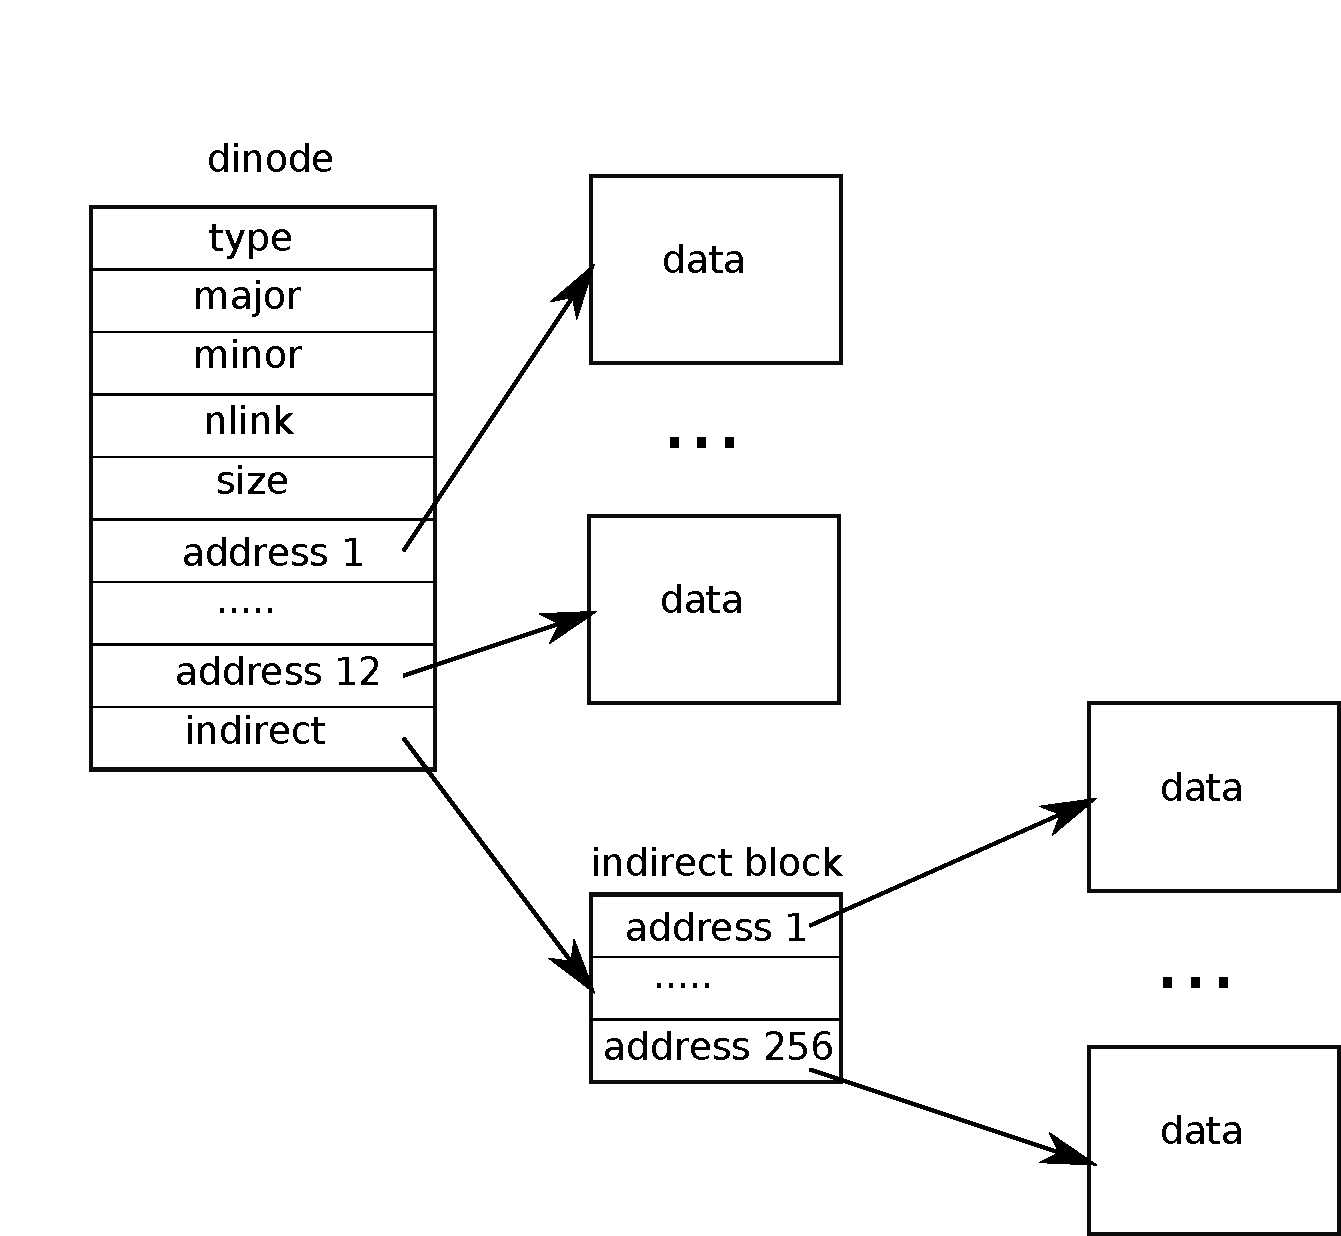
\includegraphics[scale=0.5]{fig/inode.pdf}
\caption{磁盘上文件的表示。  }
\label{fig:inode}
\end{figure}     

磁盘上的 inode 结构,
    \indexcode{struct dinode}    ,包含大小和块编号数组(参见图~    \ref{fig:inode}    )。 inode 数据可在列出的块中找到
    \lstinline{dinode}    的
    \lstinline{addrs}    数组。首先
 第一个列出了    \indexcode{NDIRECT}    数据块
 数组中的    \lstinline{NDIRECT}    条目;这些块被称为
    \indextext{direct blocks}    。下一个
    \indexcode{NINDIRECT}    数据块不在索引节点中列出,而是在称为
    \indextext{indirect block}    。最后一个条目在
    \lstinline{addrs}    数组给出间接块的地址。因此前 12 kB (
    \lstinline{NDIRECT}   
    \lstinline{x}   
    \indexcode{BSIZE}    )文件的字节可以从 inode 中列出的块加载,而下一个
    \lstinline{256}    kB (
    \lstinline{NINDIRECT}   
    \lstinline{x}   
    \lstinline{BSIZE}    )字节只能在查阅间接块后加载。这是一种很好的磁盘表示形式,但对于客户端来说却很复杂。功能
    \indexcode{bmap}    管理表示,以便更高级别的例程,例如
    \indexcode{readi}    和
 我们很快就会看到    \indexcode{writei}    不需要管理这种复杂性。
    \lstinline{bmap}    返回磁盘块号
    \lstinline{bn}    '索引节点的数据块
    \lstinline{ip}    。如果
    \lstinline{ip}   还没有这样的块,
    \lstinline{bmap}    分配 1。  

功能
    \indexcode{bmap}   
    \lineref{kernel/fs.c:/^bmap/}    首先选择简单的情况:第一个
    \indexcode{NDIRECT}    块在 inode 本身中列出
    \linerefs{kernel/fs.c:/^..if.bn.<.NDIRECT/,/^..}/}。下一个
    \indexcode{NINDIRECT}    块列在间接块中
    \lstinline{ip->addrs[NDIRECT]}    。
    \lstinline{bmap}    读取间接块
    \lineref{kernel/fs.c:/bp.=.bread.ip->dev..addr/}    然后从块内的正确位置读取块号
    \lineref{kernel/fs.c:/a.=..uint\*.bp->data/}    。如果区块数量超过
    \lstinline{NDIRECT+NINDIRECT}    ,
    \lstinline{bmap}    Panic;
    \lstinline{writei}    包含防止这种情况发生的检查
    \lineref{kernel/fs.c:/off...n...MAXFILE.BSIZE/}    。  

   \lstinline{bmap}    根据需要分配块。一个
    \lstinline{ip->addrs[]}    或间接条目为零表示未分配任何块。作为
    \lstinline{bmap}    遇到零,它用新鲜块的数量替换它们,按需分配
    \linerefs{kernel/fs.c:/^....if..addr.=.*==.0/,/./}   
    \linerefs{kernel/fs.c:/^....if..addr.*NDIRECT.*==.0/,/./}    。  

   \indexcode{itrunc}    释放文件的块,将索引节点的大小重置为零。
    \lstinline{itrunc}   
    \lineref{kernel/fs.c:/^itrunc/}    首先释放直接块
    \linerefs{kernel/fs.c:/^..for.i.=.0.*NDIRECT/,/^..}    /},然后是间接块中列出的
    \linerefs{kernel/fs.c:/^....for.j.=.0.*NINDIRECT/,/^....}    /},最后是间接块本身
    \linerefs{kernel/fs.c:/^....bfree.*NDIRECT/,/./}    。  

   \lstinline{bmap}    使之变得容易
    \indexcode{readi}    和
    \indexcode{writei}    获取 inode 的数据。
    \lstinline{readi}   
    \lineref{kernel/fs.c:/^readi/}    首先确保偏移量和计数不超出文件末尾。从文件末尾开始读取会返回错误
    \linerefs{kernel/fs.c:/^..if.off.>.ip->size/,/./}    从文件末尾开始或越过文件末尾的读取返回的字节数少于请求的字节数
    \linerefs{kernel/fs.c:/^..if.off.\+.n.>.ip->size/,/./}    。主循环处理文件的每个块,将数据从缓冲区复制到
    \lstinline{dst}   
\linerefs{kernel/fs.c:/^..for.tot=0/,/^..}    /}。
    \indexcode{writei}   
    \lineref{kernel/fs.c:/^writei/}    等同于
    \indexcode{readi}    ,有三个例外:从文件末尾开始或越过文件末尾的写入增大文件,直至最大文件大小
    \linerefs{kernel/fs.c:/^..if.off.\+.n.>.MAXFILE/,/./}    ;循环将数据复制到缓冲区而不是输出
    \lineref{kernel/fs.c:/memmove.*bp->data/}    ;如果写入扩展了文件,
    \indexcode{writei}    必须更新其大小
\linerefs{kernel/fs.c:/^..if.n.>.0./,/^..}    /}。  

功能
    \indexcode{stati}   
\lineref{kernel/fs.c:/^stati        \(/}将 inode 元数据复制到
\lstinline{stat} 结构,通过以下方式向用户程序公开
\indexcode{stat}系统调用。
\section{代码:目录层   }     

目录的内部实现与文件非常相似。它的索引节点有类型
    \indexcode{T_DIR}    及其数据是目录条目的序列。每个条目都是一个
    \indexcode{struct dirent}   
    \lineref{kernel/fs.h:/^struct.dirent/}     { 
56   } ,包含名称和索引节点号。名字最多是
    \indexcode{DIRSIZ}    (14) 个字符;如果较短,则以 NULL (0) 字节终止。 inode 号为零的目录条目是免费的。  

函数
    \indexcode{dirlookup}   
    \lineref{kernel/fs.c}     { 
552   }  在目录中搜索具有给定名称的条目。如果找到一个,它返回一个指向相应 inode 的指针,解锁并设置
    \lstinline{*poff}    到目录中条目的字节偏移量,以防调用者希望编辑它。如果
    \lstinline{dirlookup}    找到具有正确名称的条目,它会更新
    \lstinline{*poff}    并返回通过以下方式获得的解锁 inode
    \indexcode{iget}    。
    \lstinline{dirlookup}    的原因是
    \lstinline{iget}    返回未锁定的索引节点。来电者已锁定
    \lstinline{dp}    ,所以如果查找的是
    \indexcode{.}    ,当前目录的别名,尝试在返回之前锁定inode会尝试重新锁定
    \lstinline{dp}    和死锁。 (还有更复杂的死锁场景,涉及多个进程和
    \indexcode{..}    ,父目录的别名;
    \lstinline{.}    不是唯一的问题。)调用者可以解锁
    \lstinline{dp}    然后锁定
    \lstinline{ip}    ,确保它一次只持有一把锁。  

功能
    \indexcode{dirlink}   
    \lineref{kernel/fs.c:/^dirlink/}  将具有给定名称和 inode 编号的新目录条目写入目录
    \lstinline{dp}    。如果该名称已经存在,
    \lstinline{dirlink}    返回错误
    \linerefs{kernel/fs.c:/Check.that.name.is.not.present/,/^..}/} 。主循环读取目录条目以查找未分配的条目。当它找到一个时,它会提前停止循环
    \linerefs{kernel/fs.c:/^....if.de.inum.==.0/,/./} ,与
    \lstinline{off}    设置为可用条目的偏移量。否则,循环结束于
    \lstinline{off}    设置为
    \lstinline{dp->size}    。无论哪种方式,
 然后,   \lstinline{dirlink}    通过在偏移处写入来向目录添加一个新条目
    \lstinline{off}   
    \section{代码:路径名   }     

路径名查找涉及一系列调用
    \indexcode{dirlookup}    ,每个路径组件一个。
    \lstinline{namei}   
    \linerefs{kernel/fs.c:/^..strncpy/,/panic/}  评估
    \lstinline{path}   并返回相应的
    \lstinline{inode}    。功能
    \indexcode{nameiparent}    是一个变体:它在最后一个元素之前停止,返回父目录的 inode 并将最终元素复制到
    \lstinline{name}    。两者都调用广义函数
    \indexcode{namex}    来做真正的工作。  

   \lstinline{namex}   
   \lineref{kernel/fs.c:/^namex/}  首先决定路径评估从哪里开始。如果路径以斜杠开头,则从根开始求值;否则,从当前目录开始      \indexcode{skipelem}    依次考虑路径的每个元素
   \linerefs{kernel/fs.c:/..if.\*path.==....\)        /,/idup/}     。循环的每次迭代都必须查找
 当前 inode 中的    \lstinline{name}   
    \lstinline{ip}    。迭代从锁定开始
    \lstinline{ip}    并检查它是否是一个目录。如果没有,则查找失败
    \linerefs{kernel/fs.c:/^....ilock.ip/,/^....}    /}。 (锁定
    \lstinline{ip}    是必要的,不是因为
    \lstinline{ip->type}    可以在脚下改变——它不能——但是因为直到
    \indexcode{ilock}    运行,
 不保证    \lstinline{ip->type}    已从磁盘加载。)如果调用是
    \indexcode{nameiparent}    这是最后一个路径元素,循环提前停止,根据定义
    \lstinline{nameiparent}    ;最终路径元素已被复制到
    \lstinline{name}   ,所以
    \indexcode{namex}   只需返回解锁的
    \lstinline{ip}   
    \linerefs{kernel/fs.c:/^....if.nameiparent/,/^....}    /}。最后,循环使用以下命令查找路径元素
    \indexcode{dirlookup}    并通过设置为下一次迭代做准备
    \lstinline{ip = next}   
    \linerefs{kernel/fs.c:/^....if..next.*dirlookup/,/^....ip.=.next/}    。当循环耗尽路径元素时,返回
    \lstinline{ip}    。  

步骤
    \lstinline{namex}    可能需要很长时间才能完成:它可能涉及多个磁盘操作来读取路径名中遍历的目录的 inode 和目录块(如果它们不在缓冲区高速缓存中)。 Xv6 经过精心设计,因此如果调用
    \lstinline{namex}    被一个内核线程阻塞在磁盘 I/O 上,查找不同路径名的另一个内核线程可以同时进行。
    \lstinline{namex}    分别锁定路径中的每个目录,以便不同目录中的查找可以并行进行。  

这种并发带来了一些挑战。例如,当一个内核线程正在查找路径名时,另一个内核线程可能会通过取消链接目录来更改目录树。潜在的风险是查找可能正在搜索已被另一个内核线程删除的目录,并且其块已被重新用于另一个目录或文件。  

Xv6 避免了这样的竞争。例如,执行时
    \lstinline{dirlookup}    中
    \lstinline{namex}    ,查找线程持有目录的锁并且
    \lstinline{dirlookup}    返回一个使用以下方法获得的 inode
    \lstinline{iget}    。
    \lstinline{iget}    增加 inode 的引用计数。仅在收到来自的索引节点后
    \lstinline{dirlookup}    确实
    \lstinline{namex}    释放目录上的锁。现在另一个线程可能会取消该 inode 与目录的链接,但 xv6 还不会删除该 inode,因为该 inode 的引用计数仍然大于零。  

另一个风险是僵局。例如,
    \lstinline{next}    指向与以下相同的 inode
 查找“.”时的    \lstinline{ip}   。锁定
    \lstinline{next}    释放锁之前
    \lstinline{ip}    会导致死锁。为了避免这种僵局,
    \lstinline{namex}    在获取锁定之前解锁目录
    \lstinline{next}    。在这里我们再次看到为什么两者之间的分离
    \lstinline{iget}    和
    \lstinline{ilock}    很重要。
    \section{文件描述符层  }     

Unix 界面的一个很酷的方面是,Unix 中的大多数资源都以文件的形式表示,包括控制台、管道等设备,当然还有真实的文件。文件描述符层是实现这种一致性的层。  

Xv6 为每个进程提供了自己的打开文件表或文件描述符,正如我们在 Chapter~\ref{CH:UNIX}    中看到的那样。每个打开的文件都由一个表示
    \indexcode{struct file}   
    \lineref{kernel/file.h:/^struct.file/}    ,它是一个 inode 或一个管道的包装器,加上一个 I/O 偏移量。每次致电
    \indexcode{open}    创建一个新的打开文件(一个新的
    \lstinline{struct}   
    \lstinline{file}    ):如果多个进程独立打开同一个文件,不同的实例将有不同的 I/O 偏移量。另一方面,单个打开的文件(相同
    \lstinline{struct}   
    \lstinline{file}    )可以在一个进程的文件表中多次出现,也可以在多个进程的文件表中出现。如果使用一个进程就会发生这种情况
    \lstinline{open}    打开文件,然后使用创建别名
    \indexcode{dup}    或与孩子分享
    \indexcode{fork}    。引用计数跟踪对特定打开文件的引用数量。文件可以打开以进行读取或写入或两者兼而有之。这
    \lstinline{readable}    和
    \lstinline{writable}    字段对此进行跟踪。  

系统中所有打开的文件都保存在一个全局文件表中,
    \indexcode{ftable}    。文件表具有分配文件(    \indexcode{filealloc}    )、创建重复引用(    \indexcode{filedup}    )、释放引用(    \indexcode{fileclose}    )以及读写数据(    \indexcode{fileread}    和
    \indexcode{filewrite}   )。  

前三个遵循现在熟悉的形式。
    \lstinline{filealloc}   
    \lineref{kernel/file.c:/^filealloc/}    扫描文件表以查找未引用的文件 (    \lstinline{f->ref}   
    \lstinline{==}   
    \lstinline{0}    )并返回一个新的引用;
    \indexcode{filedup}   
    \lineref{kernel/file.c:/^filedup/}    增加引用计数;并且
    \indexcode{fileclose}   
    \lineref{kernel/file.c:/^fileclose/}    减少它。当文件的引用计数达到零时,
    \lstinline{fileclose}    根据类型释放底层管道或索引节点。  

功能
    \indexcode{filestat}    ,
    \indexcode{fileread}    和
    \indexcode{filewrite}    实现
    \indexcode{stat}    ,
    \indexcode{read}    和
 对文件的    \indexcode{write}    操作。
    \lstinline{filestat}   
    \lineref{kernel/file.c:/^filestat/}    仅允许在 inode 和调用上
    \indexcode{stati}    。
    \lstinline{fileread}    和
    \lstinline{filewrite}    检查打开模式是否允许该操作,然后将调用传递给管道或 inode 实现。如果文件代表一个 inode,
    \lstinline{fileread}    和
    \lstinline{filewrite}    使用 I/O 偏移量作为操作的偏移量,然后向前推进
    \linerefs{kernel/file.c:/readi/,/./}   
    \linerefs{kernel/file.c:/writei/,/./}    。管道没有偏移的概念。回想一下,inode 函数需要调用者处理锁定
    \linerefs{kernel/file.c:/stati/-1,/iunlock/}   
    \linerefs{kernel/file.c:/readi/-1,/iunlock/}   
    \linerefs{kernel/file.c:/writei\(f/-1,/iunlock/}    。 inode 锁定有一个方便的副作用,即读取和写入偏移量会自动更新,因此同时对同一文件进行多次写入不会覆盖彼此的数据,尽管它们的写入可能最终会交错。
    \section{代码:系统调用  }     

使用较低层提供的功能,大多数系统调用的实现都是微不足道的(请参见
    \fileref{kernel/sysfile.c}    )。有一些电话值得仔细研究。  

功能
    \indexcode{sys_link}    和
    \indexcode{sys_unlink}    编辑目录,创建或删除对 inode 的引用。它们是使用交易的力量的另一个很好的例子。
    \lstinline{sys_link}   
    \lineref{kernel/sysfile.c:/^sys_link/}    首先获取其参数,两个字符串
    \lstinline{old}    和
    \lstinline{new}   
    \lineref{kernel/sysfile.c:/argstr.*old.*new/}    。假设
    \lstinline{old}    存在且不是目录
    \lstinline{sys_link}    增加其
    \lstinline{ip->nlink}    计数。然后
    \lstinline{sys_link}    调用
    \indexcode{nameiparent}    查找父目录和最终路径元素
    \lstinline{new}   
    \lineref{kernel/sysfile.c:/nameiparent.new/}    并创建一个指向的新目录条目
    \lstinline{old}    的 inode
    \lineref{kernel/sysfile.c:/\|\| dirlink/}    。新的父目录必须存在并且与现有 inode 位于同一设备上:inode 编号仅在单个磁盘上具有唯一含义。如果出现这样的错误,
    \indexcode{sys_link}    必须返回并递减
    \lstinline{ip->nlink}    。  

事务简化了实现,因为它需要更新多个磁盘块,但我们不必担心更新的顺序。他们要么全部成功,要么一无所获。例如,没有交易,更新
    \lstinline{ip->nlink}    在创建链接之前会将文件系统暂时置于不安全状态,并且其间的崩溃可能会导致严重破坏。有了交易,我们就不必担心这个问题。  

   \lstinline{sys_link}    为现有 inode 创建新名称。功能
    \indexcode{create}   
    \lineref{kernel/sysfile.c:/^create/}    为新索引节点创建新名称。它是三个文件创建系统调用的概括:
    \indexcode{open}    与
    \indexcode{O_CREATE}    标志创建一个新的普通文件,
    \indexcode{mkdir}    创建一个新目录,并且
    \indexcode{mkdev}    创建一个新的设备文件。喜欢
    \indexcode{sys_link}    ,
    \indexcode{create}    通过调用开始
    \indexcode{nameiparent}    获取父目录的 inode。然后它调用
    \indexcode{dirlookup}    检查名称是否已存在
    \lineref{kernel/sysfile.c:/dirlookup.*[^=]=.0/}    。如果这个名字确实存在的话
    \lstinline{create}    的行为取决于它用于哪个系统调用:
    \lstinline{open}    具有不同的语义
    \indexcode{mkdir}    和
    \indexcode{mkdev}    。如果
    \lstinline{create}    正在代表使用
    \lstinline{open}    (    \lstinline{type}   
    \lstinline{==}   
    \indexcode{T_FILE}    )并且存在的名称本身就是一个常规文件,那么
    \lstinline{open}    认为这是成功的,所以
    \lstinline{create}    也是如此
    \lineref{kernel/sysfile.c:/^......return.ip/}    。否则,这是一个错误
    \linerefs{kernel/sysfile.c:/^......return.ip/+1,/return.0/}    。如果该名称尚不存在,
    \lstinline{create}    现在分配一个新的 inode
    \indexcode{ialloc}   
    \lineref{kernel/sysfile.c:/ialloc/}    。如果新的 inode 是一个目录,
    \lstinline{create}    初始化它
    \indexcode{.}    和
    \indexcode{..}    条目。最后,现在数据已正确初始化,
    \indexcode{create}   可以将其链接到父目录
    \lineref{kernel/sysfile.c:/if.dirlink/}    。
    \lstinline{create}    ,例如
    \indexcode{sys_link}    ,同时持有两个 inode 锁:
    \lstinline{ip}    和
    \lstinline{dp}   。不存在死锁的可能性,因为 inode
    \lstinline{ip}    是新分配的:系统中没有其他进程会占用
    \lstinline{ip}    'slock 然后尝试锁定
    \lstinline{dp}    。  

使用
    \lstinline{create}    ,很容易实现
    \indexcode{sys_open}    ,
    \indexcode{sys_mkdir}    和
    \indexcode{sys_mknod}    。
    \lstinline{sys_open}   
    \lineref{kernel/sysfile.c:/^sys_open/}    是最复杂的,因为创建新文件只是其功能的一小部分。如果
    \indexcode{open}    已通过
    \indexcode{O_CREATE}    标志,它调用
    \lstinline{create}   
    \lineref{kernel/sysfile.c:/create.*T_FILE/}    。否则,它会调用
    \indexcode{namei}   
    \lineref{kernel/sysfile.c:/if..ip.=.namei.path/}    。
    \lstinline{create}    返回一个锁定的 inode,但是
    \lstinline{namei}    没有,所以
    \indexcode{sys_open}    必须锁定 inode 本身。这提供了一个方便的地方来检查目录是否仅打开用于读取,而不是写入。假设 inode 是通过一种或另一种方式获得的,
    \lstinline{sys_open}    分配一个文件和一个文件描述符
    \lineref{kernel/sysfile.c:/filealloc.*fdalloc/}    然后填写文件
    \linerefs{kernel/sysfile.c:/type.=.FD_INODE/,/writable/}    。请注意,没有其他进程可以访问部分初始化的文件,因为它仅位于当前进程的表中。  

Chapter~\ref{CH:SCHED}    在我们拥有文件系统之前就检查了管道的实现。功能
    \indexcode{sys_pipe}    通过提供创建管道对的方法将该实现连接到文件系统。它的参数是一个指向两个整数空间的指针,它将在其中记录两个新的文件描述符。然后它分配管道并安装文件描述符。
    \section{真实世界  }     

实际操作系统中的缓冲区高速缓存比 xv6 的缓冲区高速缓存复杂得多,但它具有相同的两个目的:高速缓存和同步对磁盘的访问。 Xv6 的缓冲区高速缓存与 V6 一样,使用简单的最近最少使用 (LRU) 驱逐策略;还有许多更复杂的策略可以实施,每种策略都适合某些工作负载,但不适合其他工作负载。更高效的 LRU 缓存将消除链表,而是使用哈希表进行查找并使用堆进行 LRU 驱逐。现代缓冲区高速缓存通常与虚拟内存系统集成以支持内存映射文件。  

Xv6 的日志系统效率低下。提交不能与文件系统系统调用同时发生。系统会记录整个块,即使块中仅更改了几个字节。它执行同步日志写入,一次一个块,每个写入可能需要整个磁盘旋转时间。真实的日志系统可以解决所有这些问题。  

日志记录并不是提供崩溃恢复的唯一方法。早期的文件系统在重新启动期间使用了清除程序(例如,UNIX
    \indexcode{fsck}    程序)检查每个文件和目录以及块和 inodefree 列表,查找并解决不一致之处。对于大型文件系统,清理可能需要几个小时,并且在某些情况下不可能以导致原始系统调用成为原子的方式解决不一致问题。从日志中恢复要快得多,并且在崩溃时系统调用可以原子化。  

Xv6 使用与早期 UNIX 相同的基本磁盘索引节点和目录布局;这种方案多年来一直非常持久。 BSD 的 UFS/FFS 和 Linux 的 ext2/ext3 使用本质上相同的数据结构。文件系统布局中效率最低的部分是目录,它需要在每次查找期间对所有磁盘块进行线性扫描。当目录只有几个磁盘块时,这是合理的,但对于保存许多文件的目录来说,这是昂贵的。 Microsoft Windows 的 NTFS、macOS 的 HFS 和 Solaris 的 ZFS(仅举几例)将目录实现为磁盘上平衡的块树。这很复杂,但保证了对数时间的目录查找。  

Xv6 对于磁盘故障很天真:如果磁盘操作失败,xv6 就会出现Panic。这是否合理取决于硬件:如果操作系统位于使用冗余来掩盖磁盘故障的特殊硬件之上,那么操作系统可能很少会遇到故障,因此出现Panic是可以接受的。另一方面,使用普通磁盘的操作系统应该预料到故障并更妥善地处理它们,以便一个文件中块的丢失不会影响文件系统其余部分的使用。  

Xv6 要求文件系统适合一个磁盘设备并且大小不改变。随着大型数据库和多媒体文件对存储的要求越来越高,操作系统正在开发消除“每个文件系统一个磁盘”瓶颈的方法。基本方法是将多个磁盘组合成一个逻辑磁盘。 RAID 等硬件解决方案仍然是最流行的,但当前的趋势是尽可能在软件中实现这种逻辑。这些软件实现通常允许丰富的功能,例如通过动态添加或删除磁盘来增大或缩小逻辑设备。当然,可以动态增长或收缩的存储层需要一个可以执行相同操作的文件系统:xv6 使用的固定大小的 inode 块数组在此类环境中无法正常工作。将磁盘管理与文件系统分离可能是最简洁的设计,但是两者之间的复杂接口导致一些系统(例如 Sun 的 ZFS)将它们结合起来。  

Xv6的文件系统缺乏现代文件系统的许多其他功能;例如,它缺乏对快照和增量备份的支持。  

现代 Unix 系统允许使用与磁盘存储相同的系统调用来访问多种资源:命名管道、网络连接、远程访问的网络文件系统以及监视和控制接口,例如
    \lstinline{/proc}    。而不是xv6的
    \lstinline{if}    语句
    \indexcode{fileread}    和
    \indexcode{filewrite}   ,这些系统通常为每个打开的文件提供一个函数指针表,每个操作一个,并调用函数指针来调用该调用的 inode 实现。网络文件系统和用户级文件系统提供将这些调用转换为网络 RPC 并在返回之前等待响应的功能。
    \section{练习  }     

   \begin{enumerate}


   \item   为何Panic
    \lstinline{balloc}   ? xv6还能恢复吗?   \item   为何Panic
    \lstinline{ialloc}   ? xv6还能恢复吗?   \item   为什么不
    \lstinline{filealloc}    文件用完时出现Panic?为什么这种情况更常见并且值得处理?   \item   假设对应的文件
    \lstinline{ip}    被另一个进程取消链接
    \lstinline{sys_link}    '调用
    \lstinline{iunlock(ip)}    和
    \lstinline{dirlink}    。链接会正确创建吗?为什么或者为什么不?   \item      \lstinline{create}    进行四次函数调用(一次调用
    \lstinline{ialloc}    和三个
    \lstinline{dirlink}    )它需要成功。如果有没有的话,
    \lstinline{create}    调用
    \lstinline{panic}    。为什么这是可以接受的?为什么这四个调用都不会失败?   \item      \lstinline{sys_chdir}    次调用
    \lstinline{iunlock(ip)}    之前
    \lstinline{iput(cp->cwd)}    ,可能会尝试锁定
    \lstinline{cp->cwd}   ,尚未推迟
    \lstinline{iunlock(ip)}    直到之后
    \lstinline{iput}    不会导致死锁。为什么不?   \item   实施
    \lstinline{lseek}    系统调用。配套
    \lstinline{lseek}    还将要求您修改
    \lstinline{filewrite}    用零填充文件中的漏洞 if
    \lstinline{lseek}   套
    \lstinline{off}    超越
    \lstinline{f->ip->size.}      \item   添加
    \lstinline{O_TRUNC}    和
    \lstinline{O_APPEND}    至
    \lstinline{open}    ,这样
    \lstinline{>}    和
    \lstinline{>>}    运算符在 shell 中工作。   \item   修改文件系统以支持符号链接。   \item   修改文件系统以支持命名管道。   \item   修改文件和VM系统以支持内存映射文件。  \end{enumerate}     


